\begin{frame}[allowframebreaks]{DataLoaders}
\begin{itemize}
    \item As we have previously established, Deep Learning has been made possible by large amounts of data and computational resources.
    \item An important aspect to keep in mind is the data handling:
    \begin{itemize}
        \item How do we handle large amounts of data?
        \item How do we read different components of data (from possibly different parts of our hard drive) and provide it to our training algorithms?
        \item How do we feed this data to SGD algorithms in a streamlined manner?
    \end{itemize}

    \item PyTorch provides Dataset and DataLoaders to handle data in an efficient manner.
    \item We will subclass \texttt{Dataset} to describe our own data, then hand it to a \texttt{DataLoader} for batching and shuffling.
\end{itemize}

\framebreak

\begin{itemize}
    \item Datasets in PyTorch: The \texttt{torch.utils.data.Dataset} class is an abstract base class used to define and manage datasets for training and evaluation.
    \item Custom Dataset Creation: You can create a custom dataset by subclassing \texttt{Dataset} and implementing 
    \begin{itemize}
        \item  \texttt{\_\_len\_\_()} (returns dataset size) and 
        \item \texttt{\_\_getitem\_\_()} (fetches a single data sample).
    \end{itemize}
    
    \item DataLoaders for Batching: \texttt{torch.utils.data.DataLoader} is used to load data in mini-batches, shuffle data, and utilize multiprocessing for efficiency.
    \item Built-in Datasets: PyTorch provides datasets in \texttt{torchvision.datasets}, making it easy to load common datasets like MNIST and CIFAR-10.
\end{itemize}

\framebreak

\begin{figure}
    \centering
    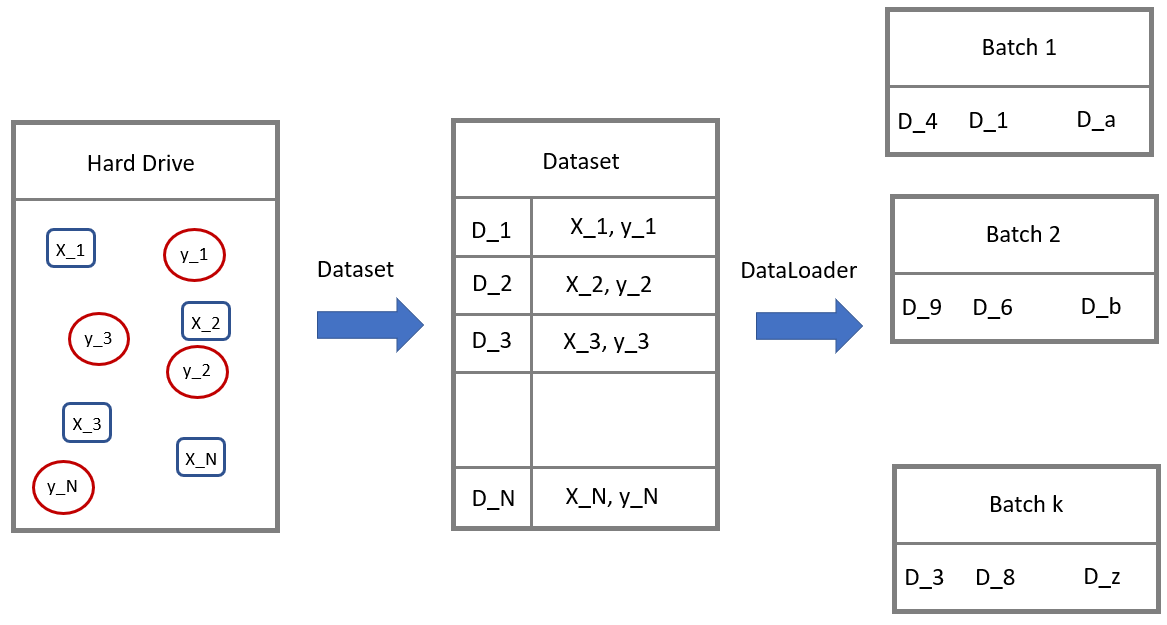
\includegraphics[width=0.5\textwidth,height=1.0\textheight,keepaspectratio]{images/dataloaders.png}
\end{figure}
\end{frame}

\begin{frame}[allowframebreaks]{A Custom Dataset and DataLoader}
    \ttfamily\footnotesize{
    from torch.utils.data import Dataset, DataLoader \\
    from torchvision import transforms \\
    from PIL import Image \\

    class ImageDataset(Dataset): \\
    \hspace{1em}    def \_\_init\_\_(self, paths, labels, transform=None): \\
    \hspace{2em}        self.paths = paths \\
    \hspace{2em}        self.labels = labels \\
    \hspace{2em}        self.transform = transform \\

    \hspace{1em}    def \_\_len\_\_(self):  \# how many samples the dataset holds \\
    \hspace{2em}        return len(self.paths) \\

    \hspace{1em}    def \_\_getitem\_\_(self, idx):  \# fetch one sample \\
    \hspace{2em}        image = Image.open(self.paths[idx]).convert("RGB") \\
    \hspace{2em}        if self.transform: \\
    \hspace{3em}            image = self.transform(image) \\
    \hspace{2em}        return image, self.labels[idx]
    }

\framebreak
    \ttfamily\footnotesize{
    to\_tensor = transforms.Compose([transforms.ToTensor()]) \\
    train\_set = ImageDataset(paths, labels, transform=to\_tensor) \\

    train\_loader = DataLoader(train\_set, batch\_size=64, shuffle=True, \\
    \hspace{9em}          num\_workers=4)
    }
\vspace{1em}
\begin{itemize}
    \item Only \texttt{\_\_len\_\_()} and \texttt{\_\_getitem\_\_()} are ours to write; \texttt{\_\_getitem\_\_()} reads one sample from disk, so nothing beyond the current batch is held in memory.
    \item The DataLoader does the rest: it groups samples into batches, reshuffles them each epoch, and reads ahead in \texttt{num\_workers} background processes so the GPU is not left waiting.
\end{itemize}
\end{frame}